\documentclass[a4paper,10pt]{article}

\usepackage[utf8]{inputenc}
\usepackage[slovene]{babel}
\usepackage{amsmath}
\usepackage{amsfonts}
\usepackage{relsize}
\usepackage[smaller]{acronym}
\usepackage{graphicx}
\usepackage{subfigure}
\usepackage{cite}
\usepackage{url}
\usepackage[unicode=true]{hyperref}
\usepackage{color}
\usepackage[version=3]{mhchem}
\usepackage{wrapfig}
\usepackage{comment}
\usepackage[left=3cm,right=3cm,top=3cm,bottom=3cm]{geometry}


%opening
\title{Hidrodinamske nestabilnosti v tankih plasteh}

\renewcommand{\vec}{\mathbf}
\newcommand{\eps}{\varepsilon}
\renewcommand{\phi}{\varphi}
\renewcommand{\theta}{\vartheta}

\newcommand{\odv}[1]{\frac{\partial #1}{\partial t}}

\newcommand{\norm}[1]{\lVert #1 \rVert}

\newcommand{\rt}{(\vec r, t)}

\begin{document}
\begin{center}

\includegraphics[width=6cm]{../logo_fmf_uni-lj_sl}\\[0.5cm]
Oddelek za fiziko \\[2cm]
{ \large Seminar -- 1. letnik, II. stopnja } \\[1cm]
{ \huge \bf Hidrodinamske nestabilnosti \\ v tankih plasteh}\\[2cm]
{\large Avtor: Miha \v Can\v cula}\\[0.6cm]
{\large Mentor: prof. dr. Alojz Kodre} \\[0.6cm]
{\large Ljubljana, marec 2012}
\end{center}
\vfill

\begin{abstract}

\end{abstract}

\newpage

\tableofcontents

\section{Uvod}

Na nestabilnosti naletimo na mnogih podro"cjih fizike. Zaradi zapletenosti ena"cb in izobilja razli"cnih pogojev so "se posebej zanimive tiste, ki izhajajo iz "studija gibanja teko"cin, hidrodinamike. 

Hidrodinamika je zelo "siroko podro"cje, ena"cbe, ki opisujejo gibanje teko"cin pa zahtevne za re"sevanje, zato se poslu"zimo dolo"cenih poenostavitev in pribli"zkov. V tem seminarju sem se posvetil le tankim plastem teko"cine. Na ta na"cin si lahko ena"cbe poenostavimo do tak"sne mere, da jim bomo znali re"siti vsaj numeri"cno, vseeno pa tudi v tako zmanj"sanem naboru sistemov najdemo veliko zanimivih problemov. Vse obravnavane primere lahko vidimo v vsakdanjem "zivljenju. 

\section{Stabilnost in zlom simetrije}

O nestabilnosti govorimo, ko infinitezimalno majhna sprememba trenutnega stanja lahko povzro"ci ve"cjo, merljivo razliko po nekem kon"cnem "casu~\cite{drazin}. 

Tak"sna definicija je precej splo"sna, zato jo za potrebe seminarja raje definiramo o"zje in bolj eksaktno. Stabilnost sistema pomeni, da vse motnje, ki so na za"cetku majhne, ostanejo majhne tudi ob poljubnem "casu. Nasprotno, sistem je nestabilen, "ce vsaj ena motnja po nekem "casu preneha biti majhna. Obi"cajno to pomeni, da "ce je motnja ob za"cetnem "casu omejena z neko zgornjo mejo, obstaja neka druga zgornja meja, ki je motnja nikoli ne prese"ze. 

"Ce se poleg stabilnosti motnja s "casom manj"sa, je tok \emph{asimptoti"cno stabilen}. V teoriji dinami"cnih sistemov asimptoti"cno stabilni re"sitvi re"cemo tudi atraktor. 

Stabilnost oz. nestabilnost sistema je tesno povezana z zlomom simetrije. Predstavljajmo si sistem, katerega "casovno spreminjanje lahko opi"semo z eno ali ve"c diferencialnimi ena"cbami, ki imajo dolo"ceno simetrijo. Z nastavkom, ki upo"steva to simetrijo, dobimo re"sitev ena"cb. Stabilnost se poka"ze, ko temu nastavku dodamo majhno motnjo, ki ne upo"steva simetrije. Stabilni sistem se bo vrnil v simetri"cno stanje, medtem ko pri nestabilnem pride do zloma simetrije. 

Primer nestabilnega pojava je svin"cnik, postavljen na konico. Ena"cba, ki opisuje njegovo gibanje, je simetri"cna glede na rotacijo okrog osi svin"cnika. Zato lahko najdemo re"sitev z enako simetrijo, to je pokon"cna lega. "Ce pa svin"cnih le malo izmaknemo iz simetri"cne lege, bo padel in kon"cal v stanju brez rotacijske simetrije. 

Po drugi strani pa je te"zno nihalo stabilen sistem. "Ce tak"sno nihalo zmotimo, bo motnja vseskozi ostajala pribli"zno majhna velika, zaradi trenja in zra"cnega upora se bo s "casom celo manj"sala. Po dolgem "caso bo sistem spet v simetri"cnem stanju. 


\section{Hidrodinamika}

\subsection{Navier-Stokesova ena"cba}

Tok nestisljive teko"cine z gostoto $\rho$ in viskoznostjo $\mu$ se podreja Navier-Stokesovi ena"cbi in ohranitvi mase. Ena"cbi za hitrost $\vec u\rt$ in tlak $p\rt$ se glasita

\begin{align}
 \label{eq:ns-enacba}
\frac{\partial \vec u}{\partial t} + \vec u \cdot \nabla \vec u &= -\frac{1}{\rho}\nabla p + \mu \Delta \vec u \\
\nabla \vec u &= 0
\end{align}

kjer je $\rho$ gostota teko"cine, $\mu$ pa njena viskoznost. 

Kot obi"cajno pri re"sevanju ena"cb si jo najprej poenostavimo tako, da preidemo na brezdimenzijske spremenljivke in "cimbolj minimiziramo "stevilo parametrov. Izberimo si meri za dol"zino $x_0$ in hitrost $v_0$. "Ce uvedemo "se brezdimenzijsko Reynoldsovo "stevilo $R=v_0 x_0 / \mu$, lahko ena"cbo zapi"semo za brezdimenzijski spremenljivki $U$ in $P$. 

\begin{align}
 \label{eq:ns-brezdim}
\frac{\partial \vec U}{\partial t} + \vec U \cdot \nabla \vec U &= -\nabla P + R^{-1} \Delta \vec U \\
\nabla \vec U &= 0
\end{align}

\subsection{Lineariziran problem}

Stabilnost hidrodinamskega sistema lahko "studiramo tako, da najprej najdemo osnovno re"sitev, ki ji v hidrodinamiki re"cemo \emph{osnovni tok}. Ta re"sitev je lahko podana analiti"cno ali numeri"cno, vsekakor pa se podreja Navier-Stokesovi ena"cbi. 

Nato osnovnem toku dodamo motnjo, tako da dobimo \emph{skupni tok}, zopet podan s hitrostjo $\vec u = \vec U + \vec u'$ in tlakom $p = P + p'$. Tudi za skupni tok mora veljati N-S ena"cba, iz "cesar lahko izpeljemo ena"cbo za motnjo $u'$ in $p'$. 

Ker nas zanimajo le majhne motnje, lahko v ena"cbi zanemarimo vse "clene kjer motnja nastopa v drugem ali vi"sjih redih. Na ta na"cin sistem zreduciramo na linearno diferecialno ena"cbo 

\begin{align}
 \label{eq:ns-linearna}
\frac{\partial \vec u'}{\partial t} + \vec U \cdot \nabla \vec u' + \vec u' \cdot \nabla \vec U &= -\nabla p' + R^{-1}\Delta u' \\
\label{eq:nestisljivost-linearna}
\nabla \cdot \vec u' &= 0
\end{align}

"Ce je osnovni tok stacionaren, so koeficienti v linearnem sistemu ena"cb konstantni, torej tak"sno ena"cba znamo re"siti. Lo"cimo lahko spremenljivki $\vec r$ in $t$, splo"sno re"sitev pa zapi"semo kot linearno kombinacijo sinusnih motenj

\begin{align}
 \vec u'\rt &= \sum e^{s_i t} \vec u_i(\vec r) \\
 p'\rt &= \sum e^{s_i t} p_i(\vec r)
\end{align}

Hitro lahko vidimo, da bo tok nestabilen, "ce ima vsaj ena lastna vrednosti $s_i$ realni del ve"cji od 0, v nasprotnem primeru pa bo stabilen. Problem stabilnosti sistema lahko torej prevedemo na iskanje lastnih vrednosti matrike. Sedaj tudi vidimo, da matemati"cno natan"cni definiciji mere za velikost motnje in kriterija za stabilnosti nimata velikega pomena, saj motnje v obliki normalnih valovnih na"cinov le eksponentno nara"s"cajo ali padajo, njihova oblika pa ostaja enaka. 

\section{Teko"cina na klancu}

Hidrodinamsko nestabilnost lahko opazujemo pri polzenju teko"cine po klan"cini~\cite{kondic}. Ta pojav je vsem dobro znan, saj ga lahko vidimo na avtomobilskih steklih v de"zju, enostavno pa je tudi pripraviti poskus doma. "Ceprav je samo re"sevanje zahteven postopek, pa lahko rezultat preverimo z eksperimentom. 

\begin{figure}[h]
\centering
 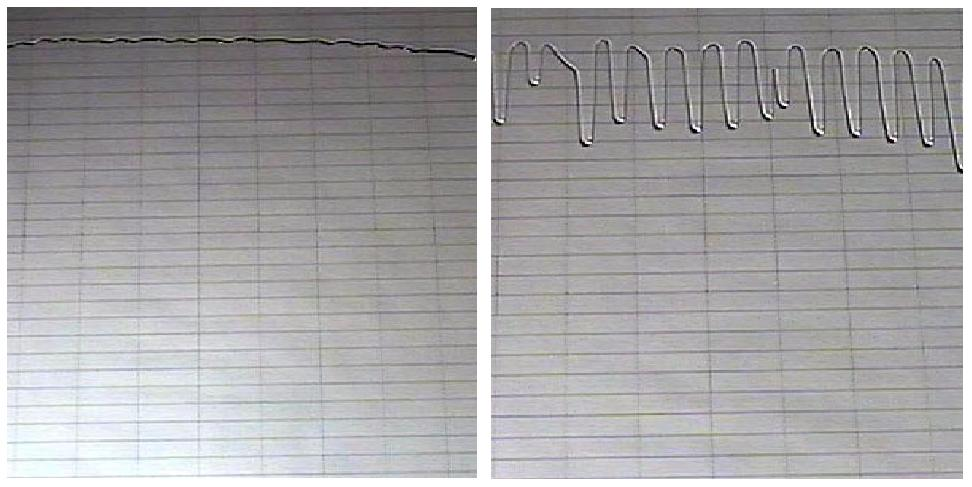
\includegraphics[width=.9\textwidth]{./Slike/film-slika}
\caption{Polzenje tanke plasti teko"cine po nagnjeni povr"sini. Majhne motnje v obliki fronte (levo) hitro prerastejo v vzorec, ki ni niti pribli"zno enakomeren, je pa periodi"cen (desno). Vir: \cite{kondic}}
\label{fig:film-neenakomernost}
\end{figure}

Vzorec na sliki~\ref{fig:film-neenakomernost} lahko pojasnimo s kratkim razmislekom. Po klan"cini navzdol vodo poganja sila te"ze, zadr"zujeta pa jo viskoznost in povr"sinska napetost, ki pa imata velik vpliv le na tanke plasti. "Ce majhna motnja ob nekem trenutku povzro"ci, da je na nekem mestu plast voda debelej"sa, imata tako viskoznost kot povr"sinska napetost manj"si vpliv na gibanje vode kot sila te"ze, zato bo na tistem mestu steklo ve"c vode kot drugod, kar bo le okrepilo za"cetno motnjo, tako da bo na tistem mestu voda vedno la"zje tekla. 

Le z razmislekom pa ne znamo napovedati niti kon"cne oblike fronte niti povpre"cne razdalje med mesti z ve"cjim pretokom. "Ce nas to zanima, moramo tudi kaj izra"cunati. 

\subsection{Ena"cbe}

"Ce privzamemo nestisljivost teko"cine $\nabla \cdot \vec u = 0$, se Navier-Stokesova ena"cba za teko"cino na klan"cu poenostavi v 

\begin{align}
 \label{eq:ns-film}
 \frac{\partial \vec u}{\partial t} + (\nabla \cdot \vec u) &= -\frac{1}{\rho}\nabla p + \frac{\mu}{\rho}\nabla^2 \vec u + g (\sin \alpha \vec i - \cos \alpha \vec k)
\end{align}

kjer je $\vec u$ hitrost teko"cine, $\rho$ njena gostota in $\mu$ viskoznost. "Clena z $g$ sta dinami"cna in stati"cna komponenta sile te"ze. Pomembni so tudi robni pogoji, obi"cajno se izbere slede"ce:

\begin{itemize}
 \item Na meji med teko"cino in klancem teko"cina ne drsi, torej je tam $\vec u = 0$. 
 \item Na meji med teko"cino in zrakom ima tlak nezveznost, ki jo sorazmerja povr"sinski napetosti in ukrivljenosti meje $\kappa$. 
\end{itemize}

Ker obravnavamo tanke filme, lahko privzamemo, da je debelina $h$ manj"sa od katerekoli dol"zinske skale v ravnini. S tem privzetkom lahko ena"cbo (\ref{eq:ns-film}) poenostavimo v ena"cbo za $h$. 

\begin{align}
\label{eq:ns-film-h}
 \frac{\partial h}{\partial t} = -\frac{1}{3\mu}\nabla \cdot \left[ \gamma h^3 \nabla \nabla^2 h - \rho g h^3 \nabla h \cos \alpha + \rho g h^2 \sin \alpha \vec i \right]
\end{align}

\begin{figure}[h]
\centering
 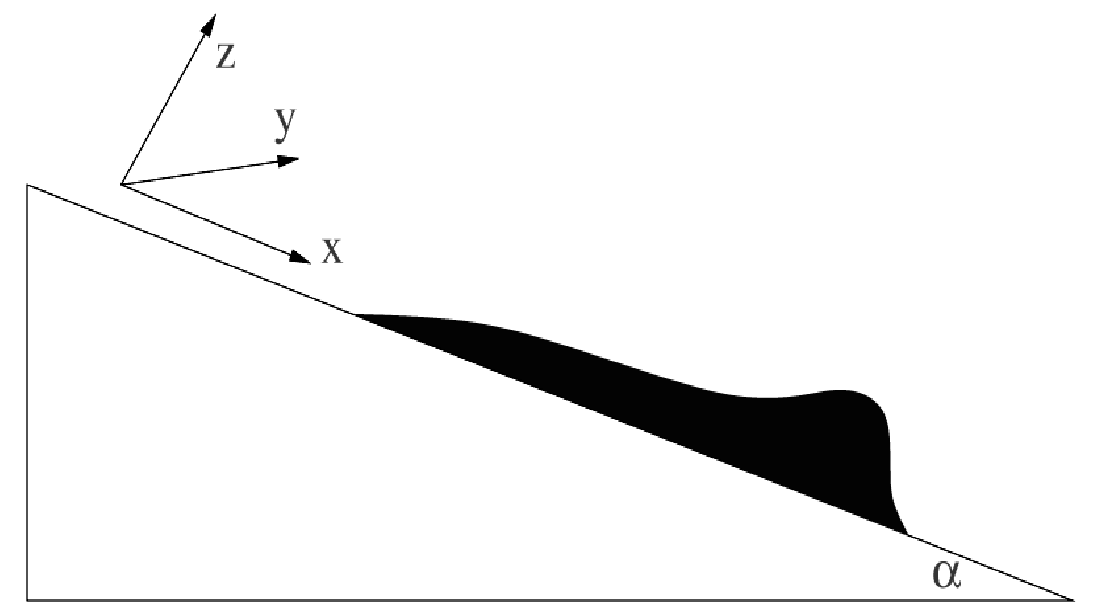
\includegraphics[width=.8\textwidth]{./Slike/film-skica}
\caption{Skica teko"cine v dveh dimenzijah. Viden je greben tik za fronto teko"cine in pa zo"zitev dale"c za fronto, ki je pri ra"cunih ne bomo upo"stevali}
\label{fig:film-skica}
\end{figure}

Da najdemo osnovno re"sitev, najprej privzamemo, da ima re"sitev enako simetrijo kot sama ena"cba. Postavimo se v koordinatni sistem kot na sliki~\ref{fig:film-skica}. Klanec, po katerem te"ce teko"cina, ima translacijsko simetrijo v smeri $y$, zato za osnovno re"sitev velja $h_y = 0$. "Za la"zje re"sevanje preidemo "se na brezdimenzijske koli"cine. V ena"cbi ostane le "se en parameter $D(\alpha)$, ki podaja razmerje med vplivom viskoznostji in povr"sinske napetosti, brezdimenzijsko dol"zino klanca v smeri $x$ pa ozna"cimo z $L$. Ena"cba za brezdimenzijske koli"cine, ki predpostavlja simetrijo in zato opisuje osnovno re"sitev problema, se glasi

%% TODO: Mogoce bi vseeno napisal kaksna je substitucija v brezdimenzijske?

\begin{align}
  \label{eq:ns-film-sim}
 \odv{h} &= - \left[h^3 h_{xxx}\right]_x + D(\alpha) \left[h^3 h_x\right]_x - \left(h^3\right)_x
\end{align}

Pred za"cetkom re"sevanja moramo dolo"citi tudi za"cetne in robne pogoje. Ena"cba je "cetrtega reda v $x$, zato potrebujemo "stiri robne pogoje. "Ce za"cnemo s podobnim profilom kot na sliki~\ref{fig:film-skica}, le da se rep nadaljuje do zgornjega roba klan"cine, velja $h(0, t) = 1$ po definiciji brezdimenzijse debeline, pred fronto pa je plast mnogo tanj"sa, $h(L, t) = b \ll 1$. Oba enakosti ne veljata le na robu obmo"cja, ampak tudi v njegovi bli"zini, zato za ostala dva robna pogoja vzamemo $h_x(0,t) = h_x(L,t) = 0$. Potrebujemo "se za"cetni pogoj, ki je kar profil teko"cine ob "casu $t=0$. Naravna izbira je krivulja, ki povezuje dva ravna odseka z gladkim vmesnim delom. 

\subsection{Re"sevanje}

Zgornja ena"cba je "se vedno prezahtevna, da bi jo re"sevali analiti"cno, zato pose"zemo po numeri"cnih metodah. Re"sitev ena"cbe (\ref{eq:ns-film-sim}) lahko dobimo z uporabo metode na osnovi kon"cnih diferenc. Ena"cba je prvega reda v "casu in "cetrtega reda v koordinati $x$, zato je najbolj pomembna izbira diskretizacije za $x$. Najve"c pozornosti moramo posvetiti diskretizaciji najvi"sjega "clena v ena"cbi, ki je v na"sem primeru "cetrtega reda. 

\begin{figure}[h]
 \centering
 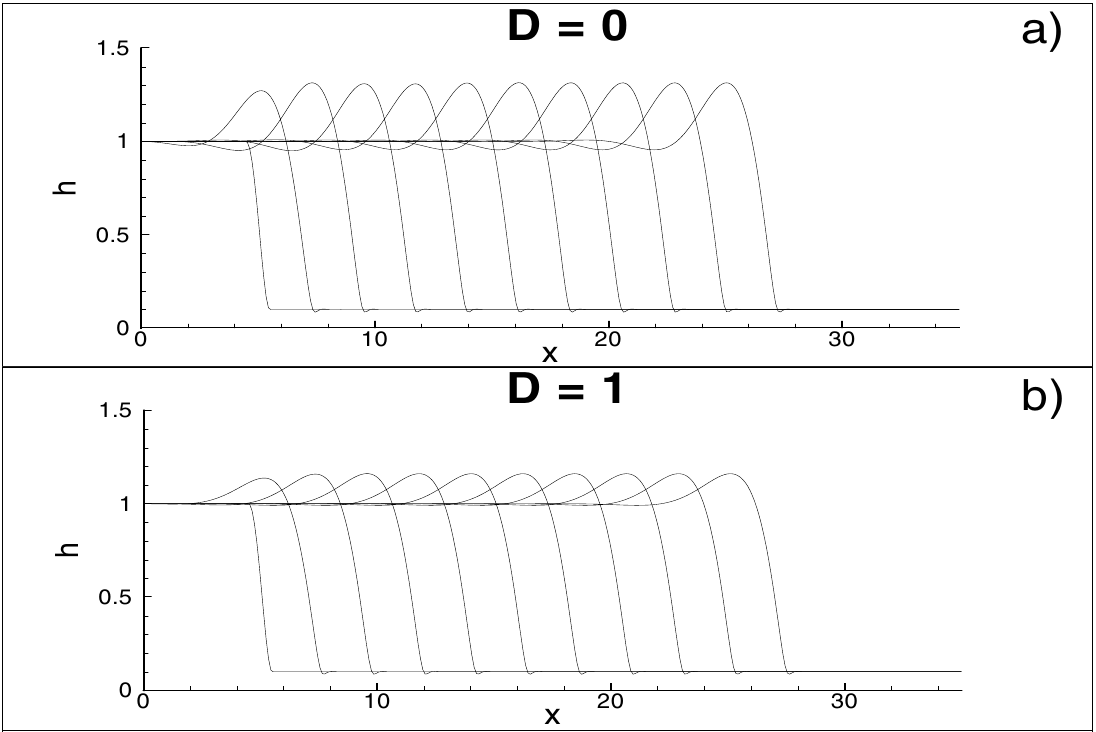
\includegraphics[width=.8\textwidth]{./Slike/film-osnovna-resitev}
 \caption{Profil teko"cine pri razli"cnih vrednostih parametra $D$. V obeh primerih se hitro oblikuje greben tik za fronto. Profili so prikazani v intervalih $\delta t = 2$, pri izbranih vrednostih $L = 40$ in $b=0,1$. Koordinata $x$ je diskretizirana s korako $\Delta x = 0,05$~\cite{kondic}. }
 \label{fig:film-osnovna}
\end{figure}


\subsection{Nestabilnost}

Osnovna re"sitev $h_0(x, t)$ je sicer odvisna od "casa, vendar lahko predpostavimo, da rob teko"cine polzi s konstantno hitrostjo $U$. "Casovno odvisnost koeficientov $h_0$ bomo torej odpravili, "ce se postavimo v koordinatni sistem, ki se giblje s to hitrostjo. V tem primeru uvedemo spremenljivko $\xi = x - Ut$ in $\nabla = (\partial_\xi, \partial_y)$, splo"sno re"sitev pa lahko zapi"semo v obliki

\begin{equation}
 h(\xi, y, t) = h_0(\xi) + \eps h_1(\xi, y, t)
\end{equation}

V tej sliki se $h_0$ ne spreminja s "casom, torej smo dobili linearno diferencialno ena"cbo s konstantnimi koeficienti. Ker "zelimo, da je motnja res majhna, predpostavimo, da sta $h_0$ in $h_1$ podobnega velikostnega reda, $\eps$ pa zelo majhen, dosti manj"si od 1. Zgornji izraz vstavimo v ena"cbo (\ref{eq:ns-film-h}) in zanemarimo vse "clene z drugi in vi"sjimi potencami $\eps$. 

Motnjo $h_1$ izberemo tak"sno, da zanjo ne dr"zi translacijska simetrija v smeri $y$. Na sliki~\ref{fig:film-neenakomernost} vidimo, da je oblika fronte pribli"zno periodi"cna, zato $h_1(\xi, y, t)$ raje zapi"semo kot linearno kombinacijo normalnih valovnih na"cinov. V ena"cbi bo tako nastopala Fourierova transformiranka po koordinati $y$, ki jo ozna"cimo z $g(\xi, q, t)$, za katero velja

\begin{align}
 \odv{g} = -\mathcal{L}g
\end{align}

Tu je $\mathcal{L}$ linearni diferecialni operator s konstantimi koeficienti. Zanimajo nas lastne vrednosti tega operatorja, zlasti tista z najve"cjim realnim delom. Lastne vrednosti so odvisne od valovnega "stevila $q$ oz valovne dol"zine $\lambda = 2\pi/q$; pri"cakujemo, da bo valovna dol"zina, pri kateri je lastna vrednost $s(q)$ najve"cja, enaka razdalji med posameznimi pasovi na sliki~\ref{fig:film-neenakomernost}, saj bo motnja s tak"sno valovno dol"zino najhitreje nara"s"cala. 

Ker smo osnovno re"sitev $h_0$ izra"cunali numeri"cno, tudi matri"cne elemente operatorja $\mathcal{L}$ poznamo le numer"cno. 

\begin{figure}[h]
 \centering
 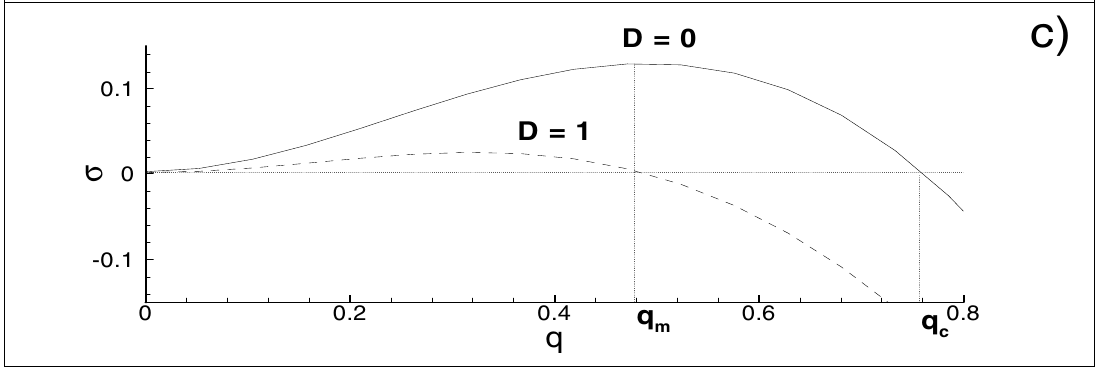
\includegraphics[width=.8\textwidth]{./Slike/film-stabilnost}
 \caption{Hitrost rasti $\sigma$ majhne motnje z valovnim "stevilom $q=2\pi/\lambda$. Na"cin z najhitrej"so rastjo $q_m$ ustreza pri"cakovani razdalji med vzorci.~\cite{kondic}. }
 \label{fig:film-osnovna}
\end{figure}

\section{Milni mehur"cki}

\begin{figure}[h]
 \centering
\subfigure{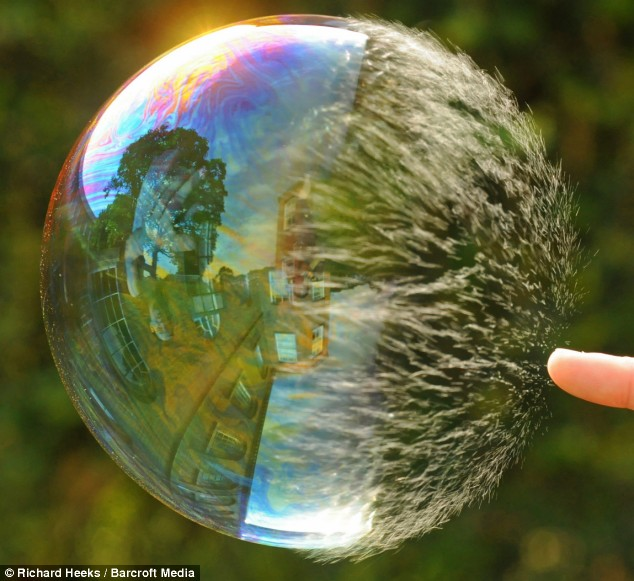
\includegraphics[height=.45\textwidth]{./Slike/bubble-3}}
\subfigure{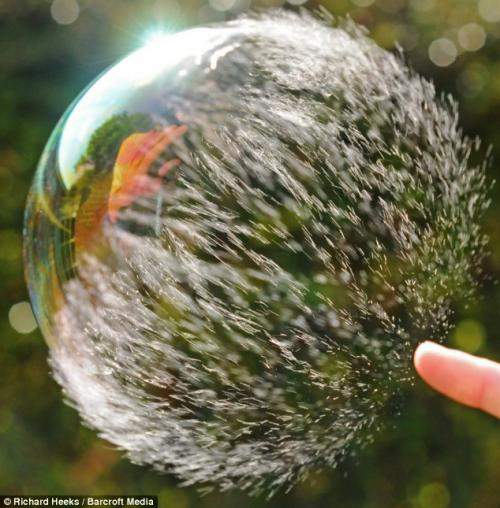
\includegraphics[height=.45\textwidth]{./Slike/bubble-4}}
\caption{Razpad milnega mehur"cka~\cite{slike-mehurcek}. }
\label{fig:mehurcek-3}
\end{figure}

Milni mehur"cki so stabilni na majhne motnje zaradi povr"sinske napetosti teko"cine. "Ce pa mehur"cek predremo v eni to"cki, ustvarimo rob, kjer povr"sinska napetost ni uravnote"zena, zato se rob za"cne umikati. Ker je opna obi"cajno zelo tanka, je ukrivljenost na robu velika, zato fronta napreduje zelo hitro~\cite{diploma}. To napredovanje je pri mehur"ckih tako hitro, da s prostim o"cesom fronte sploh ne opazimo, ampak se nam zdi, da celoten mehur"cek razpade naenkrat. Pri opazovanju si lahko pomagamo s hitrimi kamerami, kot vidimo na sliki~\ref{fig:mehurcek-3}. 

Podobno kot pri tankem filmu tudi tu obravnavamo tanko plast teko"cine pod vplivom povr"sinske napetosti. Skica roba opne z ozna"cenimi spremenljivkami in koordinatnimi osmi je na sliki~\ref{fig:mehurcek-skica}. 
\begin{figure}[h]
 \centering
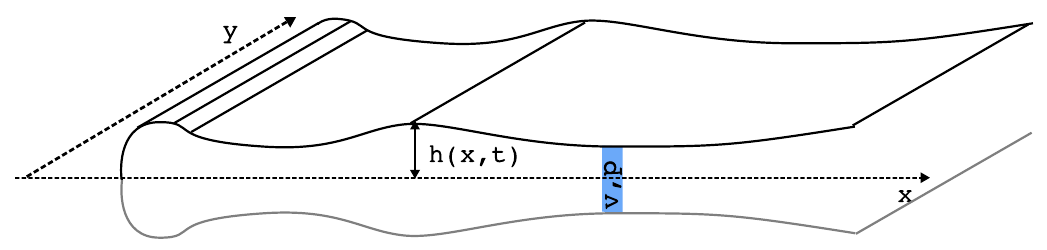
\includegraphics[width=.8\textwidth]{./Slike/mehurcek-skica}
\caption{Profil opne s translacijsko simetrijo vzdol"z roba in zrcalno simetrijo v navpi"cni smeri. Ker je opna tanka, lahko privzamemo, da se tlak in hitrost ne spreminjata po debelini~\cite{diploma}. }
\label{fig:mehurcek-skica}
\end{figure}

Pojava pa se mo"cno razlikujeta v viru nestabilnosti. Pri razpadu milnega mehur"cka namre"ce ne opazimo nestabilnosti v obliki fronte, ampak v dejstvu, da opna razpade v kapljice. Pravzaprav gre za zloma dveh simetrij, ene v smeri premikanja fronte in druge v pravokotni smeri. Re"sevanje problema je mnogo la"zje ob predpostavki, da se translacijska simetrija vzdol"z roba ohranja, torej se osredoto"cimo le na prvi zlom simetrije. Kljub temu pa so ena"cbe "se vedno prezapletene za analiti"cno re"sevanje, zato pose"zemo po numeri"cnih metodah. 

S pomo"cjo simulacije lahko napovemo velikost in hitrost kapljic, ki se odcepijo od opne. Rezultat simulacije, ki jo je za diplomsko nalogo izvedel Simon "Copar, je na sliki~\ref{fig:mehurcek-rez-1}. 

\begin{figure}[h]
  \centering
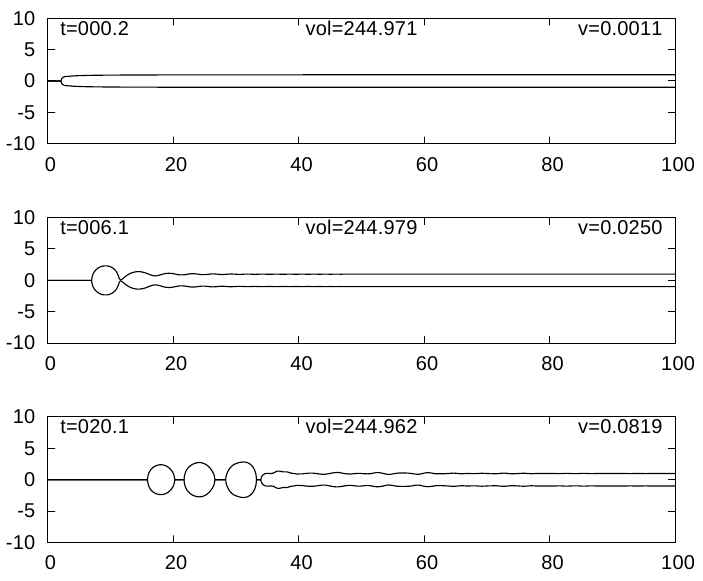
\includegraphics[width=.8\textwidth]{./Slike/mehurcek-rezultat-1}
\caption{"Casovno spreminjanje roba opne med razpadom milnega mehur"cka. Vidno je premikanje fronte in tvorba kapljic s polmerom, ki je dosti ve"cji od debeline opne.~\cite{diploma} }
\label{fig:mehurcek-rez-1}
\end{figure}

\begin{figure}[h]
  \centering
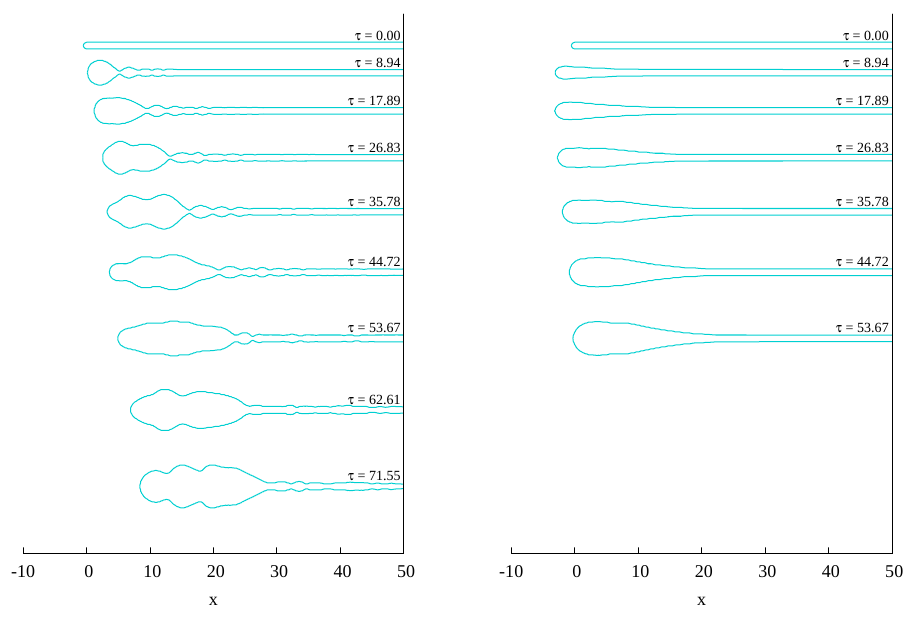
\includegraphics[height=200pt]{./Slike/scat-rezultat-1}
\caption{Spreminjanje roba opne, ki je dovolj viskozna, da prepre"ci razpad v kapljice.~\cite{scat} }
\label{fig:mehurcek-rez-1}
\end{figure}

Dobljena parametra lahko preverimo, saj se morata ohranjati tako skupna energija kot tudi celotna prostornina. Skupena prostornina opne in vseh kapljic je izra"cunana na sliki~\ref{fig:mehurcek-rez-1}, med tekom simulacije pa se spremeni za manj kot en promil. Podoben izra"cun lahko naredimo tudi za skupno energijo kapljic in opne, le da moramo tu se"steti ve"c prispevkov. Energija je lahko v obliki povr"sinske napetosti, kineti"cne energije ali nihanja kapljic. 


Tok neviskozne in nestisljive teko"cine opisuje Eulerjeva ena"cba

\begin{equation}
\label{eq:meh-euler}
 \odv{\vec v} + (\vec v \cdot \nabla)\vec v = - \nabla p
\end{equation}

Hkrati pa za opno velja tudi ohranitev prostornine, ki jo v brezdimenzijski obliki zapi"semo kot

\begin{equation}
\label{eq:meh-ohranitev}
 \odv{h} + \nabla (h\vec v) = 0
\end{equation}

Vemo, da opna za fronto razpade v kapljice. Njihovo "stevilo in velikost lahko dolo"cimo iz ohraniev energije in skupne prostornine. Pred razpadom je edini prispevek k energiji povr"sinska napetost opne, po razpadu pa nastane $N$ enako velikih kapljic z radijem $r$ in hitrostjo $v$. Ohranitev energije ob razpadu odseka opne s povr"sino $S$ da enakost

\begin{equation}
 \sigma N 4 \pi r^2 + 2 S h_0 \rho \frac{v^2}{2} = 2S\sigma
\end{equation}

kjer je prvi "clen energija povr"sinske napetosti kapljic, drugi kineti"cna energija kapljic, na desni pa energija opne pred razpadom. Zvezo med povr"sino opne $S$ in "stevilom kapljic $N$ dobimo iz ohranitve volumna, tako da se ohranitev energije v brezdimenzijski obliki, kjer je $r$ v enotah $h_0$, $v$ pa v enotah $v_0 = \sqrt{\frac{\sigma}{\rho h_0}}$, glasi

\begin{equation}
 \frac{3}{r} + \frac{v^2}{2} = 1
\end{equation}

Drugo zvezo med velikostjo in hitrostjo kapljic pa dobimo ob predpostavki, da fronta s "casom ohranja svojo obliko, torej jo lahko zapi"semo kot potujo"ci val. Ker se premika le v eni smeri, uporabimo valovno ena"cbo prvega reda

\begin{equation}
 \frac{\partial v}{\partial t} + c \nabla v = 0
\end{equation}

"Ce bi bila hitrost valovanja $c$ manj"sa od hitrosti teko"cine na robu $v$, bi bilo gibanje teko"cine nadzvo"cno in bi nastajali udarni valovi. "Ce pa bi bila motnja hitrej"sa od teko"cine, bi opna razpadala "ze pred fronto. Edina smiselna mo"znost je torej, da je $c=v$. 

Primerjava s posnetki razpadov resni"cnih milnih mehur"ckov ni povsem primerna, saj ne moremo narediti mehur"cka iz neviskozne teko"cine. 

\section{Kra"ski "zlebi"ci}

% TODO: Citat, dobi diplomo od Kodreta

\begin{figure}[h]
\centering
 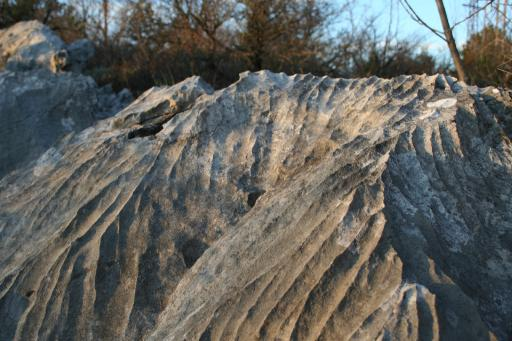
\includegraphics[width=.8\textwidth]{./Slike/Zlebici}
 \caption{"Zlebi"ci na slovenskem Krasu pri Nabre"zini~\cite{wiki:zlebic} }
 \label{fig:zlebici-slika}
\end{figure}

S slike~\ref{fig:zlebici-slika} lahko vidimo, da "zlebi"ci tvorijo podobno periodi"cno strukturo kot teko"cina na sliki~\ref{fig:film-neenakomernost}. Tudi po izvoru sta pojava sorodna: Na tistih mestih, kjer "cez "zlebi"c ste"ce ve"c vode, se tudi raztopi ve"c apnenca, torej postane kanal "se globlji in skozenj te"ce "se ve"c vode. Plast teko"cine tu seveda ni tako tanka, da bi povr"sinka nepotest igrala veliko vlogo, je pa "se vedno debelina toka $h$ dosti manj"sa od velikosti pobo"cja, na katerem se tvorijo "zlebi"ci. 

\begin{figure}
 \centering
  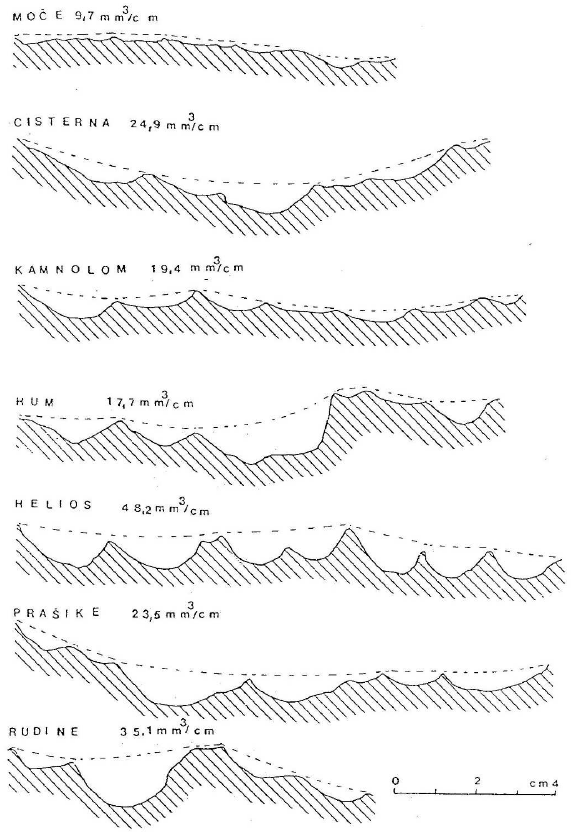
\includegraphics[height=250pt]{./Slike/zlebici-profil}
  \caption{Nekaj zabele"zenih profilov "zlebi"cev~\cite{gams}}
\end{figure}


Proces tvorbe "zlebi"cev je dosti bolj zapleten kot zgoraj obravnavani primeri. Namesto znane kon"cne koli"cine vode imamo sedaj neenakomeren de"z, pa tudi pobo"cje ni nujno ravno in homogeno. Kakr"snekoli ra"cune "se posebej ote"zi raztapljanje apnenca v vodi, zapleten kemijski proces ki "se vedno ni natan"cno pojasnjen. Znane Navier-Stokesove ena"cba so zato sklopljene z ena"cbami za raztapljanje, ki so znane le empiri"cno. Vse kra"ske kamnine so zelo slabo topne v vodi, zato so tak"sni procesi prepo"casni, da bi lahko z njimi izvajali fizikalne eksperimente, pomagamo si lahko le s "stevilnimi primeri "zlebi"cev najdenih v naravi.

Zaradi teh omejitev lahko nastanek in razvoj "zlebi"cev modeliramo le s simulacijo. Pri tem moramo narediti kar nekaj poenostavitev, upo"stevamo pa lahko opa"zanja iz narave. 

Nastanek "zlebi"cev na nekem skalnatem pobo"cju je neposredna posledica nestabilnosti. V simulaciji torej opazujemo, kaj se dogaja z majhno motnjo. V ta namen za"cnemo z "zlebi"cem, katerega globina je majhna v primerjavi s "sirino in dol"zino. "Ce se tak "zlebi"c s "casom poglobi, lahko zaklju"cimo, da je povr"sina pobo"cja nestabilna, saj se majhne motnje s "casom ve"cajo. 

\section{Razpad curka}

Na nestabilnosti pogosto naletimo tudi pri "studiju razpada curkov teko"cin~\cite{eggers}. 

\section{Zaklju"cek}

\begin{thebibliography}{3}
  \bibitem{drazin} P. G. Drazin, \textit{Introduction to hydrodynamic stability}, Cambridge University Press (2002)
  \bibitem{kondic} L. Kondic, SIAM Review \textbf{45}, 95 (2003)
  \bibitem{slike-mehurcek} \url{http://www.dailymail.co.uk/sciencetech/article-1199149/Super-slow-motion-pictures-soap-bubble-bursting-stunning-detail.html} (23. 1. 2012)
  \bibitem{diploma} S. "Copar, Numeri"cna analiza nestabilnosti na robu teko"cinske opne, Diplomsko delo (2009)
  \bibitem{wiki:zlebic} \href{http://sl.wikipedia.org/wiki/\%C5\%BDlebi\%C4\%8Di}{http://sl.wikipedia.org/wiki/\v Zlebič} (2. 2. 2012)
  \bibitem{gams} I. Gams, Geografija in aktualna vpra"sanja prostorskega razvoja, 127--138 (1989)
  \bibitem{eggers} J. Eggers in E. Villermaux, Rep. Prog. Phys. \textbf{71}, 036601 (2008)
  \bibitem{scat} L. J. Gordillo Zavaleta, Self-similar and travelling wave solutions in surface tension-driven thin planar films, Scientific Computing Advanced Training (2007)
\end{thebibliography}


\end{document}
